\documentclass{article}

%%%%%%%%%%%%%%%%%%%%%%%%%%%%%%%%%%
%%%%%%%%%%%% Packages %%%%%%%%%%%%
%%%%%%%%%%%%%%%%%%%%%%%%%%%%%%%%%%
\usepackage{graphicx, svg}
\usepackage[font={small,it}]{caption}
\usepackage{tikz}
\usepackage{quiver}
\usepackage{esdiff}

% math packages
\usepackage{amsmath}
\usepackage{amsthm}
\usepackage{amsfonts, dsfont}
\usepackage[T1]{fontenc}
\usepackage{mathtools, extpfeil}

% for better cross-reference workflow
%\usepackage{showlabels}
\usepackage[bookmarks=True]{hyperref}
\usepackage{bookmark}
\renewcommand{\arraystretch}{1.5}

% for better list and enumeration
\usepackage[shortlabels]{enumitem}

% to-do notes
\usepackage{todonotes}

% Removes paragraph indent and adds spacing between paragraphs
\usepackage[parfill]{parskip} 
\usepackage{setspace}

% darkmode
\usepackage{darkmode}
%\enabledarkmode

%%%%%%%%%%%%%%%%%%%%%%%%%%%%%%%%%%%%%
%%%%%%%%%%%% Environment %%%%%%%%%%%%
%%%%%%%%%%%%%%%%%%%%%%%%%%%%%%%%%%%%%

\newtheorem{thm}{Theorem}
\newtheorem{cor}[thm]{Corollary}
\newtheorem{lem}[thm]{Lemma}
\newtheorem{pro}[thm]{Proposition}

\theoremstyle{definition}
\newtheorem{re}[thm]{Remark}
\newtheorem{defn}[thm]{Definition}
\newtheorem{ex}[thm]{Example}

%%%%%%%%%%%%%%%%%%%%%%%%%%%%%%%%
%%%%%%%%%%%% Symbol %%%%%%%%%%%%
%%%%%%%%%%%%%%%%%%%%%%%%%%%%%%%%
\newcommand{\Z}{{\mathbb Z}}
\newcommand{\C}{{\mathbb C}}
\newcommand{\R}{{\mathbb R}}
\newcommand{\N}{{\mathbb N}}
\newcommand{\Q}{{\mathbb Q}}
\newcommand{\qand}{\quad \text{and} \quad}

\newcommand{\dive}{div}
\newcommand{\grad}{\operatorname{grad}}
\newcommand{\curl}{\operatorname{curl}}
\newcommand{\F}{\mathbf{F}}
\newcommand{\dist}{\operatorname{dist}}
\newcommand{\erf}{\operatorname{Erf}}

\renewcommand{\div}{\operatorname{div}}
\renewcommand{\i}{\mathbf{i}}
\renewcommand{\j}{\mathbf{j}}

\newcommand{\pd}{+\dots+}
\newcommand{\many}{,\dots, }
\newcommand{\ten}{\otimes}

%%%%%%%%%%%%%%%%%%%%%%%%%%%%%%%%%%%%%
%%%%%%%%%%%% New Command %%%%%%%%%%%%
%%%%%%%%%%%%%%%%%%%%%%%%%%%%%%%%%%%%%

% Rounded brackets
\newcommand{\br}[1]{\left(#1\right)}

% Curly Brackets
\newcommand{\sbr}[1]{\left\{#1\right\}}

% Functions
\newcommand{\func}[2]{#1 \br {#2}}

% Inverse functions
\newcommand{\invfunc}[3]{#1^{-#2} \br {#3}}

% Compact list
\setlist[itemize]{itemsep=3pt, topsep=2pt}
\setlist[enumerate]{itemsep=3pt, topsep=2pt}

%%%%%%%%%%%%%%%%%%%%%%%%%%%%%%
%%%%%%%%%%%% Size %%%%%%%%%%%%
%%%%%%%%%%%%%%%%%%%%%%%%%%%%%%
\usepackage{geometry}
\geometry{a4paper, margin=1in}

%%%%%%%%%%%%%%%%%%%%%%%%%%%%%%
%%%%%%%%%% Spacing %%%%%%%%%%%
%%%%%%%%%%%%%%%%%%%%%%%%%%%%%%
\setlength{\parskip}{0.5\baselineskip} 
\setlength{\parindent}{0pt}

\title{MH4110 Presentation Notes: Deriving Maxwell's Equations}
\author{Wee Lun}
\date{25 Feb 2026}

\begin{document}

\maketitle

\begin{abstract}
    The Maxwell's equations are a set of four fundamental equations that describe the behavior of electric and magnetic fields. They were formulated by James Clerk Maxwell in the 19th century and are essential for understanding electromagnetism. The equations can be derived from a combination of experimental observations and mathematical principles.
\end{abstract}

\section{Basic Notation and Motivation}

Recall the following definition from Calculus 3:

\medskip

\begin{defn} [Vector field]
    A vector field is a function that assigns a vector to each point in a subset of space. Mathematically, a vector field $\F$ on a subset $S$ of $\R^n$ can be expressed as: 
    \[\F: S \to \R^m\]
\end{defn}

In the study of electromagnetism, two important vector fields are the electric field $E$ and the magnetic field $B$, which both can be considered as vector fields defined in three-dimensional space mapping to $\R^3$.
\begin{itemize}
    \item Electric field $E$ represents the force experienced by a charged particle in the presence of other charges.
    \item Magnetic field $B$ represents the force experienced by a moving charged particle in the presence of other moving charges or magnetic materials.
\end{itemize}
Recall that $\nabla\cdot $ represents the $\div$ operator, which measures the vector field's tendency to originate from or converge into a point. On the other hand $\nabla \times$ represents the $\curl$ operator, which measures the rotation of a field. 
\begin{figure}[h]
    \centering
    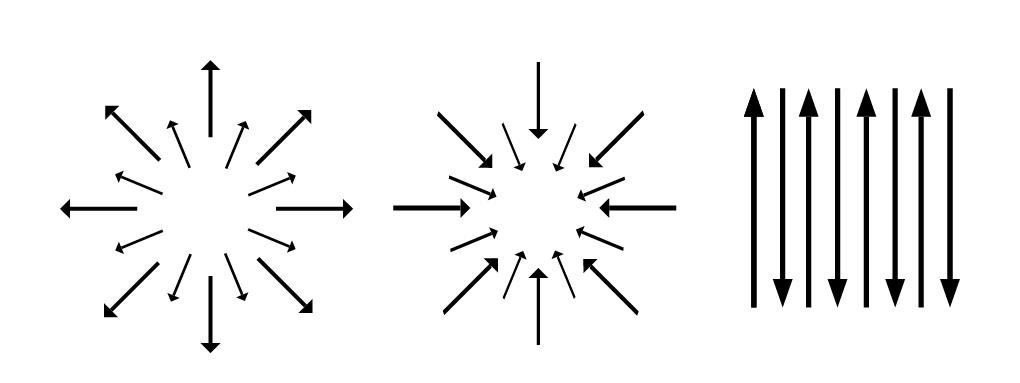
\includegraphics[scale=0.3]{div.jpeg}
    \footnotesize{\caption{In the first image, we see the vector field is diverging from a point, giving $\nabla\cdot \F >0$. The second image shows the field is converhing to a point, this gives $\nabla \cdot \F <0$. The last image does not show any tendency of converging and diverging, thus $\nabla\cdot F = 0$}}
\end{figure}

We are particular interested in the divergence and the curl of a vector field due to the \textit{Helmholtz Decomposition Theorem} (i.e. Fundamental Theorem of Vector Calculus), where the theorem provides a method to uniquely decompose a vector field, under some condition, into the sum of two components: an irrotational (curl-free) part and a solenoidal (divergence-free) part. In other words, the theorem says that, under some condition, a vector field can be described entirely using $\curl$ and $\div$, allowing us to study the vector field structurally.

Of course, Helmholts Decomposition Theorem is applicable to electric field and magentic field, which motivates us to study the divergence and curl of electric fields, and magnetic fields. These quantities are, unsurprisingly, described by the Maxwell's Equations.

\section{Derivation of Maxwell's Equations}

Considering the spacetime as $\R^3\times \R$. We will be deriving the following set of equations in this handout:

\medskip

\begin{defn} [Maxwell's Equations]
    Maxwell's equations is given by the following set of equations:
    \[\nabla\cdot E = \frac{\rho}{\epsilon_0}\]
    \[\nabla\cdot B = 0\]
    \[\nabla\times E = -\frac{\partial B}{\partial t}\]
    \[\nabla\times B = \mu_0 \br{J + \epsilon_0\frac{\partial E}{\partial t}}\]
    where \begin{itemize}
        \item $E, B:\R^3\times \R \to \R^3$ are eletric field and magnetic field respectively. 
        \item $\rho:\R^3\times \R \to \R$ is the charge density, i.e. the amount of electric charge per unit length
        \item $J: \R^3 \times \R\to \R^3$ is the current density, i.e. the amount of chanrge per unit time that flows through a unit area of a chosen cross section
        \item Both $\epsilon_0$ and $\mu_0$ are constant. The formal one is the vacuum permitivity, which determines electric field strength per unit charge density; the later one is the vacuum permeability, which determines magnetic response to current.
    \end{itemize}
\end{defn}
The name for each of the equation is, from top to bottom, Gauss' Law, Gauss' Law for magnetism, Maxwell-Faraday's Law, and Ampère-Maxwell Law. As mentioned previously $\nabla\cdot$ and $\nabla \times$ are the $\div$ and $\curl$ operator respectively, thus Maxwell's Equations allow us to describe the divergence and curl of electric field $E$ and magnetic field $B$.

Before starting the derivation of each equation, we shall briefly describe our starting point:
\begin{enumerate}
    \item Coulumb's Law is used to derive Gauss' Law.
    \item Biot-Savant Law is used to derive the Gauss' Law for magnetic.
    \item Faraday's Law is used to derived the Maxwell-Faraday's Law.
    \item Ampère's Law and the Charge Conservation Law are used to derive the Ampère-Maxwell Law.
\end{enumerate}

\begin{re}
    The speed of the electromagnetic waves, is given by 
    \[c = \frac{1}{\sqrt{\epsilon_0 \mu_0}}\]
\end{re}

\subsection{Gauss' Law}

\subsection{Gauss' Law for Magenetic}

\subsection{Maxwell-Faraday's Law}

\subsection{Ampère-Maxwell Law}

\section{Discussion and Analysis}

In fact, Charge Conservation Law can be derived from Maxwell's Equations:

\medskip 

\begin{thm} [Charge Conservation Law]
    We have the following transport equation:
    \[\partial_t \rho + \nabla\cdot J = 0\]
\end{thm}
\begin{proof}
    Recall Ampère-Maxwell's Equation is given by
    \[\nabla \times B = \mu_0 \br{J + \epsilon_0 \diffp{E}{t}}\]
    Taking divergence $\nabla\cdot$ both sides gives
    \[0 = \nabla\cdot (\nabla\times B) = \nabla\cdot \br{\mu_0 \br{J + \epsilon_0 \diffp{E}{t}}} = \mu_0 \br{\nabla\cdot J + \epsilon_0 \diffp{}{t} (\nabla\cdot E)}\]
    where the equality at LHS is due to the vector calculus identity that divergence of a curl field is $0$ (one can verify by expanding out the definition of div and curl). The equality at RHS is due to commutativity of operator $\diffp{}{t}$ and $\nabla\cdot$. Lastly, by applying Gauss' Law $\nabla\cdot E = \dfrac{\rho}{\epsilon_0}$, we get 
    \[\mu_0\br{\nabla\cdot J + \epsilon_0 \frac{1}{\epsilon_0}\diffp{\rho}{t}} = 0 \implies \nabla\cdot J + \diffp{\rho}{t} =0\]
    This proves the identity.
\end{proof}

This demonstrates that Maxwell's equations imply charge conservation. However, note that this proof is merely a interesting consequence of Maxwell's equations, rather than a standard common proof of local charge consevation, as the standard proof does not rely on Maxwell's equation.

\end{document}